\documentclass[12pt]{article}
\usepackage{amsfonts}
\usepackage{mathrsfs}
\usepackage{booktabs}
\usepackage{graphicx}
\usepackage{subfigure}
%\usepackage{bbm}
\usepackage{color}
\usepackage{amsmath}
\usepackage{cases}
\newcounter{mytempeqncnt}
\usepackage{amssymb}
\pagestyle{empty} \textwidth 17cm \textheight 22.5cm
\renewcommand{\baselinestretch}{1.2}
\newcommand{\BOX}{\hfill $\Box$}
\newcommand{\NAB}{\hfill $\nabla \nabla \nabla$}
\newcommand{\BYDEF}{\stackrel{\rm \Delta}{=}}
\newcommand{\bm}[1]{\mbox{\boldmath{$#1$}}}
\topmargin -2.0cm \oddsidemargin 0.0cm \evensidemargin 0.0cm
\parskip 0.3cm
\parindent 0.0cm
\baselineskip 0.5cm \makeatletter
\def\EquationsBySection{\def\theequation{\thesection.\arabic{equation}}%
\@addtoreset{equation}{section}}
\def\TheoremsBySection{\def\thetheorem{\thesection.\arabic{theorem}}%
\@addtoreset{theorem}{section}}
\def\DefinitionsBySection{\def\thedefinition{\thesection.\arabic{definition}}%
\@addtoreset{definition}{section}}
\def\RemarksBySection{\def\theremark{\thesection.\arabic{remark}}%
\@addtoreset{remark}{section}}
\def\LemmasBySection{\def\thelemma{\thesection.\arabic{lemma}}%
\@addtoreset{lemma}{section}}
\def\AssumptionsBySection{\def\theassumption{\thesection.\arabic{assumption}}%
\@addtoreset{assumption}{section}} \makeatother
\newcommand{\ba}{\begin{array}}
\newcommand{\ea}{\end{array}}
\newcommand{\be}{\begin{equation}}
\newcommand{\ee}{\end{equation}}
\newcommand{\bea}{\begin{eqnarray}}
\newcommand{\eea}{\end{eqnarray}}
\newcommand{\bc}{\begin{center}}
\newcommand{\ec}{\end{center}}
\newcommand{\hs}{\hspace}
\newcommand{\vs}{\vspace}
\newcommand{\lt}{\left}
\newcommand{\rt}{\right}
\newcommand{\bib}{\bibitem}
\newcommand{\ds}{\displaystyle}
\newcommand{\fc}{\frac}
\newcommand{\nm}{\nonumber}
\newcommand{\ol}{\overline}
\newcommand{\da}{\Delta}
\newcommand\old[1]{}
\newtheorem{remark}{Remark}
\EquationsBySection \TheoremsBySection \DefinitionsBySection
\RemarksBySection \LemmasBySection \AssumptionsBySection
\begin{document}
\begin{flushright}
     Dr. Zhixin Liu \\
    Institute of Electrical Engineering\\
    Yanshan University \\
    Qinhuangdao, 066004 China  \\
    E-mail: lzxauto@ysu.edu.cn
    \\
    %\today
\end{flushright}
\begin{flushleft}
Professor Syrotiuk\\
Area Editor\\
Computer Networks



\end{flushleft}
Dear Editor,\\

Thank you very much for your email and the review comments on our
paper:
\begin{center}
{\bf Ref.  Number COMNET\_2018\_612}\\
{``Energy efficient resource allocation based on relay
selection and subcarrier pairing with channel
uncertainty in cognitive radio network"}
\end{center}
which was required MAJOR revisions before resubmission. Please find the
substantially revised paper, which is ready for publication in
\emph{Computer Networks}.

As kindly suggested by you and the reviewers, the paper has been
seriously revised in accordance to the constructive and helpful
comments from you and the reviewers for improving the quality
further. All the modifications in the revision have been marked \textcolor{red}{in
red}. For more information, please see the detailed Responses to the
Reviewers.

We would like to express our sincere appreciation to you for your
prompt and professional handling of our manuscript.

Looking forward to hearing from you.

Yours sincerely,

\vspace{3mm} Zhixin Liu


\newpage
\pagestyle{plain}
\title{\Huge{Responses to Reviewers\thanks{For the paper, Ref.  Number COMNET\_2018\_612, ``nergy efficient resource allocation based on relay selection and subcarrier pairing with channel
uncertainty in cognitive radio network," submitted to {\em Computer Networks}.}}}
\author{}
\date{}
\maketitle We would like to thank the reviewers for their careful
assessments and constructive comments on our submission,
particularly the time being spent. We take the reviewers' views very
seriously, and have made every possible effort in order to address
the concerns raised by the reviewers and modify the paper according
to his/her suggestions and comments. We have corrected all the
errors and typos. The details are explained below.

We hope this revised version is now suitable for publication in {\bf
Computer Networks}.\\

\newpage

{\Large \underline{Response to Reviewer 1}}

We would like to thank the reviewer for spending his/her time to assess the paper, and make very constructive and detailed informative comments provided in the review.
Our responses are given as follows:

\begin{enumerate}
%R1Q1
\item \textbf{Question}: Although it can be readable, the quality of the manuscript needs to be improved. For instance, the authors study the cognitive-radio relay network, but they do not state clearly in the section of introduction that the cognitive-radio relay networks will be studied in this manuscript.

\textbf{Answer}: Thanks for the reviewer's suggestions! We have added some reviews about the cognitive-radio relay network in the revision. In addition, at the end of the introduction, the interference management of cognitive wireless networks also are discussed. The revised part is marked {in red} in the revision, and some of them are as follows.

``With the tremendously increasing demands on high speed wireless communications, more and more spectrum
resources are required. In order to make full use of limited spectrum resources, cognitive radio network has emerged.
But, when the distance between the destination node and the source node is far away or there is occlusion,
the communication between the nodes will be seriously affected. In order to ensure the normal communication
of the destination node, the assisted transmission of the cognitive relay is an efficient way. Cognitive relay-
assisted communication also has become very popular in wireless systems, such as cognitive radio cellular, ad-hoc
networks[1]. It could promote the overall system performance by means of improving the spectral efficiency and
extending the coverage area. To fully realize these benefits in cooperative communication systems, efficient wireless
resource allocation is critical.''

`` In [10], the author presents an energy-efficient
resource allocation scheme with joint consideration of relay selection, subcarrier pairing and power allocation.
For each selected relay, one subcarrier pair containing two subcarriers is allocated to reduce the transmit power
consumption with minimum data rate guarantee. In [11], the author considers an AF-based cooperative two-hop
multi-relay OFDM system, where they optimally and jointly allocate the three types of resources: power, subcarriers
and relay nodes. The works in [12], [13], [14], [15], [16] mainly study the multi-carrier modulation under perfect
CSI knowledge. However, the channel state information can not be known precisely in the actual situation. In order
to solve the problem of spectrum shortage, the cognitive-radio relay technology is applied in the [17], [18], [19].
Compared with the previous works that did not use cognitive-radio relay technology, the utilization of spectrum
resources of the system have been improved more efficiently. But the drawback is that secondary users will suffer
more interference with the primary users.''

\item \textbf{Question}:

  a) The abbreviation CR in the abstract is not clear.

  b) The sentence ``we assume that there is only one communication link works in a time period and the topology of each secondary user is different"  has been repeated twice in the system model ( i.e., the sentence above Fig.1 and the sentence below (12)).

  c) The definition of a time period is not provided in this manuscript.

  d) In the sentence below (8), what is the meaning of mid point?

  e) In (12), 2/T should be T/2.

  f) Many sentences are quite obscure, e.g., the sentence above Fig.9, "It is obviously that the energy-efficiency of the system obtained by using the uncertain channel is greater than the energy-efficiency of the system under the assumed perfect channel in most cases, the robustness of the system with channel estimation error is greatly improved.", and the sentence "The simulation result shows that the system��s energy-efficiency is not along with the boundary of channel estimation error monotonous change, that is, not the greater the boundary of the channel estimation error is, the more obvious the performance improvement of the system��s energy-efficiency will be".

The authors are suggested to proofread the manuscript to make it more readable and understandable.


\textbf{Answer}: Thanks for the reviewer's carefulness and sorry for our negligence! We have made relevant explanations and modifications according to reviewer's requirements.

a) CR means Cognitive Radio.

b) The sentence repeated below (12) has been deleted.

c) A communication time period is denoted as $T$, and the definition has been added at the beginning of the Section II in the revision.

d) The midpoint is the median value of this line segment, this line segment contains the boundaries of the uncertain channel. The corresponding explanation has been added.

e)  $2/T$ has changed to $T/2$.

f) The sentences pointed out by the reviewer have been modified. \\
``It is obviously that the energy-efficiency of the resource allocation scheme considering the uncertain channel is greater than the scheme assuming the perfect channel(regardless of channel estimation error) can be achieved. The robustness of the system with consideration of channel estimation error is greatly improved".

``From the simulation results, it is not true that the increased channel estimation error can lead to the decreased energy efficiency. There is no consistent rule between them".

We have revised the whole manuscript carefully and tried to avoid any error.



%R1Q2
\item \textbf{Question}: In the studied network, the authors assume that there are $M$ source nodes in the cognitive multi-relay cooperative communication network. However, only the m-th source node is considered in the section of problem formulation, e.g., (12) and (17). The number of source nodes, i.e., M, cannot be found in the formulated problem. Therefore, how to determine the optimal source node is not clear in this manuscript.


\textbf{Answer}: Thanks for the reviewer's constructive suggestions and questions! In this paper, we consider DF relay mode, it is assumed that the information transmission period $T$ is divided into two identical time slots. In the first time slot, the primary user transmit information to the base station with power $P_p$, and cause the interference to the relay nodes and destination nodes. Meanwhile, the secondary user $S_m$, sharing the same frequency with the primary user, transmits its information with power $P_{sm}$ to relay nodes $R_i$, destination nodes $D_j$, and cause interference to the base station. In the second time slot, the relay nodes decode and forward the information with power $P_{ri,dj}$ to different destinations, that also causes interference to the base station. Meanwhile, the primary users also works with power $P_p$, and cause the interference to the destination nodes $D_j$. In the first time slot, the secondary users need to share the frequency band with the primary user, and each secondary user wants to occupy the available frequency band for communication. In order to ensure the fairness between the secondary users, the secondary users adopt TDMA for communication, that is, only one secondary user sends information during a communication cycle. So we only consider the case that there is only one source node, i.e. the $m$-th secondary user, and give an example to design the allocation strategy to maximize the system energy efficiency. The proposed scheme and algorithm are also applicable to other source nodes. So, all the source nodes(secondary users) can share and access the available frequency, and there is no optimal source node. If the the energy efficiency corresponding to every source node reaches the maximum, the whole maximum energy efficiency is achieved.

The corresponding explanations have been added in the revision.

%R1Q3
\item \textbf{Question}:  In the formulated problem, the author assume that the number of subcarriers is the same as that of the destination nodes. It is a quite special and ideal assumption. It is not clear that the derived results can be extended to the general scenario where the number of subcarriers and the number of the destination nodes are different.

\textbf{Answer}: Thanks for the reviewer's comment! The problem you mentioned is seriously considered in the paper. In fact, the proposed algorithm can be extended to the general scenario and the number of subcarriers and destination nodes can be different. For clarity, we set that there are $K$ subcarriers and $J$ destination nodes in the revision. \\
If the number of subcarriers is different from the number of destination nodes, there are two cases as follows.

1) $K \geq J$, when we use the Hungarian algorithm, we will use 0 to complete the remaining vacancy positions into a square matrix. This is similar to the assumption that the number of subcarriers is the same as the number of destination nodes.

2) $K<J$, that means that there are not enough subcarriers to be used by the destination nodes, and some users can not be accepted. In this case, we will remove redundant destination nodes, and this also becomes the case where the number of destination nodes is equal to the number of subcarriers.

Therefore, our assumptions are general and reasonable assumptions. In order to simplify the calculation, we assume that the number of subcarriers is the same as the number of destination nodes. The corresponding explanation has been added to the revision.

%R1Q4
\item \textbf{Question}:  In the sentence below (22), the authors state that the constraint (C:7) can only meet the requirements in the case of $P_{sm}G_{sm,b} < P_{ri,dj}^lG_{ri,b}^l$, which may cause that only the suboptimal solution can be achieved in the formulated problem. The authors should clarify on this assumption.

\textbf{Answer}: Thanks for reviewer's comment! The problem you mentioned is seriously considered in the paper. Constraint (C:7) is represented by the rate of $R_{p,b}$ in Equation (21) at two different time slots. In DF relay mode, the achieved transmission rate is determined by the minimum rate of two parts. As shown in Equation (22), $R_{p,b}$ depends on $P_{sm}G_{sm,b}$, $P_pG_{p,b}$ and $P_{ri,dj}^lG_{ri,b}^l$. It is noted that both $P_p$ and $P_{sm}$ are fixed, and $P_{ri,dj}^l$ is variable. We attempt to take a power control strategy to maximize the energy efficiency. In order to describe the piecewise function as a unified form, we consider the case only including the variable in the constraint (C:7). If we consider the situation $P_{sm}G_{sm,b}>P_{ri,dj}^lG_{ri,b}^l$, the variable $p$ is not included in the constraint. It means constraint (C:7) is not affected by the adjusted power of user and the achieved rate is limited by the first time slot. In this scenario, the system does not implement the power control strategy. The focus of our research is to adjust the power $p$ to meet the interference requirements of the primary user, and to maximize the energy efficiency of the system. So we consider the situation $P_{sm}G_{sm,b}<P_{ri,dj}^lG_{ri,b}^l$. It can meet the communication needs of the primary user, and the energy efficiency of the system will be maximized by implementing the power control strategy. Some explanations have been added in the revision.

%R1Q5
\item \textbf{Question}:  Compared with the related work in literature, the authors consider the channel estimation error in the studied CR relay network. By employing the worst case method, the reformulated problem is quite similar to that in literature, e.g. [R1], but the network studied in this manuscript is more simplified than that in [R1] since the subcarrier allocation is not performed in the first slot. The authors are suggested to further clarify the difference between their work and the related work in literature, especially on the employed optimization method.

    [R1]  Wenbing Dang, Meixia Tao, Hua Mu, and Jianwei Huang, '' Subcarrier-Pair Based Resource Allocation for Cooperative Multi-Relay OFDM Systems'', IEEE TRANSACTIONS ON WIRELESS COMMUNICATIONS, VOL. 9, NO. 5, MAY 2010.

\textbf{Answer}: Many thanks for the reviewer's valuable suggestions and questions!

1) Literature [R1] has a great correlation with our article, we quote it as the literature [26] and review it in the revision.

2) In literature [R1], the author formulates a subcarrier pairing based resource allocation problem for cooperative two-hop multi-relay OFDM systems with AF protocol. The objective is to maximize the end-to-end transmission rate subject to individual or total power constraints. And they solve the optimization problems for both individual and total power constraints using a dual method in an asymptotically optimal manner. Finally, based on the intuition derived from the optimal algorithm, they further propose two suboptimal algorithms for the problem with individual power constraints.

3) In this paper, a robust resource allocation algorithm is proposed to maximize the energy efficiency (EE) in a multi-carrier decode-and-forward (DF) relay cognitive radio(CR) network, which is different from [R1]. Moreover, unlike many of the previous works which consideredd ideal channel, we consider a dynamic channel with  channel estimation error. In addition, the robustness of the system is improved by using the worst-case method. This paper focus on the resources allocation in cognitive relay networks where the primary and secondary users share the spectrum and the robust energy-efficiency maximization algorithm is given jointly considering  power allocation, subcarrier pairing and relay selection. While the literature [R1] studies downlink in the cooperative multi-relay OFDM system. For the optimization method, although it is also the power control, subcarrier allocation and relay selection, but the literature [R1] achieves the maximum system throughput by power control, this paper uses the power control to achieve the maximum energy efficiency of the system. They are the difference between this article and the literature [R1]. Despite this, there are still many places in literature [R1] that we deserve to learn. The main contributions of this paper are as follows:

First, we not only combine subcarrier pairing, relay selection and power allocation to maximize system's energy-
efficiency, but also improve spectral efficiency through CR spectrum sharing.

Second, the original optimization problem is a non-convex fractional mixed binary integer programming problem,
i.e. NP-hard to solve, we use the Dinkelbach method to convert this problem into a linear problem and prove that this function is a convex function. And then we use standard Hungarian method to solve the NP-hard problem.

Third, the channel state information is dynamic in the actual situation. In order to get closer to the real channel, in
this paper, we formulate energy-efficiency maximization (EEM) in cognitive radio network problem, which jointly
addresses the subcarrier pairing, relay selection and power allocation under a uncertainty channel environment,
then, we use the worst-case method to convert the probabilistic constraints into the deterministic.
%R1Q6
\item \textbf{Question}:  The results in Fig.8 are quite confusing. The achieved energy efficiency with perfect channel information cannot be worse than that with statistical channel estimation error. Can the authors clarify on this point?

\textbf{Answer}: Thanks for the reviewer's valuable suggestions and comments! We are sorry for the confused expression about  ``the perfect channel''.  Here, the perfect channel refers to the ideal channel which is under the assumption that there is no channel estimation error and channel gain can be achieved precisely.  In the actual environment, it is impossible. It can be regarded as ideal case. In the simulations, it is set that the estimation errors exist and two algorithms are tested. Because the power allocation scheme under the ideal channel neglect the statistical channel estimation error, it shows worse energy efficiency. To avoid confusion, we change ``the perfect channel"  to ``the ideal channel'' in the revision and add some explanations in the revision.

 The simulation results are shown in Figure 1. It is noted that, when we do the energy efficiency with the statistical channel estimation error, the channel estimation error fluctuates above and below the ideal channel. If the dynamic channel conditions are worse than the ideal channel, the energy efficiency of the system under the dynamic channel may be lower than the ideal channel condition, such as when the threshold is $2\times10^{-9}$ in Figure 1. However, taking the uncertainty of channel gain into account, the achieved energy efficiency with statistical channel estimation error is generally superior to the ideal channel.

\begin{figure}[h]
        \centering
        \includegraphics[width=0.5\textwidth]{statistical_channel_error.eps}
        \caption{Influence of statistical channel estimation error under different boundaries on system's energy-efficiency}
        \vspace*{2mm}
        \label{fig:centralized}
\end{figure}

\end{enumerate}

Finally, thanks the reviewer again for the comments provided, and the time and efforts spent in the review. We hope that the above modifications have answered the reviewer's concerns.

\newpage

{\Large \underline{Response to Reviewer 2}}

We would like to thank the reviewer for the careful examining work and the time spent.

Our responses to the reviewer's comments are given as follows:

\begin{enumerate}
%R2Q1
\item\textbf{Question}: In the system model, the authors mentioned about CR, while in the title and contribution there is nothing about CR. The authors are suggested to refine the related parts.

\textbf{Answer}: Thanks for the reviewer's suggestions!
We have modified and title of the paper and added some contents about the cognitive radio networks in the Introduction and Conclusions in the revision. And the revised part is marked {in red}.

%R2Q2
\item\textbf{Question}: The proposed subcarrier pairing, relay selection and power allocation schemes for CR with imperfect CSI is not really novel, and the Dinkelbach method has been widely used.  For example, the resource allocation schemes are studied in ``Energy Efficient Resource Allocation for OFDMA Two-Way Relay Networks with imperfect CSI, " EURASIP Journal on Wireless Communications and Networking, 2015:225, and the energy efficiency problems have been studied in  ``Energy Efficient Resource Allocation for Wireless Power Transfer Enabled Collaborative Mobile Clouds,''  IEEE Journal on Selected Areas in Communications, vol. 34, no. 12, Dec. 2016. The authors may need to highlight their novelty.

\textbf{Answer}: Many thanks for the reviewer's valuable suggestions and questions! We agree with the reviewer that the topics about resource allocation and energy efficiency maximization are not new, however, we think there are some aspects different from the existing works in this paper. We give brief explanations as follows.

1) The above literatures have a great correlation with our paper, we quote them as the literature [21] and [22] in the revision, which are quite helpful to the part of optimization problem formulation. In literature [21], the problem of distributing cellular data via a wireless power transfer enabled collaborative mobile cloud (WeCMC) in an energy efficient manner is investigated. When considering multi-input multi-output wireless channel and wireless power transfer, an efficient algorithm is presented to optimally schedule the data offloading and radio resources in order to maximize energy efficiency as well as fairness among mobile users. The authors also propose an algorithm that can properly assign the subchannels for the transmission between the BS and WeCMC, and the transmission within WeCMC. In literature [22], the author present an energy-efficient resource allocation scheme with joint consideration of relay selection, subcarrier pairing, and power allocation under the imperfect CSI. For each selected relay, one subcarrier pair containing two subcarriers is allocated with the objective to reduce the transmit power consumption with minimum data rate guarantee.

2)In this paper, a robust resource allocation algorithm is proposed to maximize the energy efficiency (EE) in a multi-carrier decode-and-forward (DF) relay cognitive radio(CR) network. Unlike many of the previous works in the literatures which consider the ideal channel, we consider a dynamic channel with channel estimation error. Although the literature [22] also considers imperfect channels, we use different ways to handle the imperfect channel. In addition, the robustness of the system is improved by using the worst-case method in this paper. By introducing cognitive radio network to alleviate the strained spectrum. This paper researches cognitive radio networks that are shared simultaneously by primary and secondary users. Compared with other articles, this is a completely different communication scenario. The communication quality of the primary user is guaranteed and the energy efficiency of the system reaches maximum under our optimal power control algorithm. Under the intense spectrum resources, we have fully utilized the limited spectrum resources. The main contributions of this paper are summarized as follows:

First, we not only combine subcarrier pairing, relay selection and power allocation to maximize system's energy-
efficiency, but also improve spectral efficiency through CR spectrum sharing.

Second, the original optimization problem is a non-convex fractional mixed binary integer programming problem,
i.e. NP-hard to solve, we use the Dinkelbach method to convert this problem into a linear problem and prove that this function is a convex function. And then we use standard Hungarian method to solve the NP-hard problem.

Third, the channel state information is dynamic in the actual situation. In order to get closer to the real channel, in
this paper, we formulate energy-efficiency maximization (EEM) in cognitive radio network problem, which jointly
addresses the subcarrier pairing, relay selection and power allocation under a uncertainty channel environment,
then, we use the worst-case method to convert the probabilistic constraints into the deterministic.

%R2Q3
\item\textbf{Question}: The way of transforming the nonconvex problem in Sec. III. C may not be correct. It is required that eq. 19 is quasi-convex. The authors should refine it or prove it.

\textbf{Answer}: Thanks for the reviewer's valuable questions! After careful consideration, we make relevant explanations and make some supplements in the paper. The equation (19) is indeed not a form of convex function, so we use the Dinkelbach method to convert the nonlinear fractional function into the linear subtraction form. Then, referring to the literature [23], $EE = R(p) / P(p)$ is transformed into the form of $F(q^*) = R(p)-q^*P(p)$.  We can prove that the form of this subtraction is a convex function. For the fixed $q^*$, we find the second derivative of $F(q^*)$,


\begin{eqnarray}\label{41}
\begin{split}% ����һ�����,λ�ô�ֱ����
\frac{\partial{F(q^*)}}{\partial{P_{ri,dj}^l}}=\frac{g_{ri,dj}^l(e_{ri,dj})}{ln2(P_{ri,dj}^lg_{ri,dj}^l(e_{ri,dj})+P_{sm}g_{sm,dj}(e_{sm,dj})+P_pg_{p,dj}(e_{p,dj})+N_0)}-q*.
\end{split}
\end{eqnarray}

\begin{eqnarray}\label{41}
\begin{split}% ����һ�����,λ�ô�ֱ����
\frac{\partial^2{F(q^*)}}{\partial{{P_{ri,dj}^l}^2}}=\frac{(g_{ri,dj}^l(e_{ri,dj}))^2}{ln2(P_{ri,dj}^lg_{ri,dj}^l(e_{ri,dj})+P_{sm}g_{sm,dj}(e_{sm,dj})+P_pg_{p,dj}(e_{p,dj})+N_0)^2}>0.
\end{split}
\end{eqnarray}

Since the second derivative of $F(q*)$ is larger than zero, the transformed function is a convex function.

We have added the explanation in the revision.

%R2Q4
\item\textbf{Question}: It is unclear how to obtain optimal $q$ in the proposed scheme 1. In addition, there is no complexity analysis as the authors claim using proposed scheme can decrease it.

\textbf{Answer}: Thank you very much for reviewer's comment! We also appreciate the reviewer for the valuable suggestions and questions. \\
 Firstly, the Dinkelbach method is an iterative algorithm, which is able to approach the optimal solution. The introduced parameter $q$ is actually the energy efficiency. The value of $q$ updates continuously with the change of other parameters. When the energy efficiency reaches the maximum, the parameter $q^*$ is the maximum of system's energy efficiency. In the simulations, the specific solution for $q^*$ is as follows:

1)Set the maximum number of external cycles $Z$, and set the initial value of $q$ to 0.0001.

2)Initialize each parameter.

3)Set the maximum number of internal loops $T$ and enter the inner loop.

4)In the inner loop, update power $P_{ri,dj}^l$, Lagrangian multipliers $��$ and $��$ until it converges and jumps out of the inner loop.

5)In the outer loop, the converged power $P_{ri,dj}^l$, Lagrangian multipliers $��$ and $��$ are used to update the Dinkelbach coefficient $q$, the subcarrier allocation indicator and the relay selection indicator until $q$ converges and jumps out of the outer loop, at this time $q =q^*$, which is the maximum energy efficiency value.

Secondly, we have add the complexity analysis in the revision. The following is the complexity analysis of the subcarrier allocation algorithm, where $n$ represents the number of subcarriers. The worst case time complexity of the Hungarian algorithm is $O(n^3)$ and the complexity of the exhaustive method is $O(n!)$. When $n$ is large, the complexity of the EEM algorithm is lower than the exhaustive method. The complexity of the FSA (Fixed Subcarrier Allocation) method is $O(1)$, and the complexity of the CSO (Channel State Ordering) method is $O(n)$. Although the algorithm complexity of two methods is low, the obtained system performance is not good. In the objective function fraction, the numerator and denominator contain $J$ variables. We can get the optimal $q^*$ with the maximum iterations, $Z$, in the worst case. The time complexity of the Dinkelbach method is $O(log(J Z))$ in the worst case. Finally, in this paper, the complexity of the algorithm is $O(log(J Z) n^3)$.

%R2Q5
\item\textbf{Question}: The proposed scheme should prepare with the state of the art instead of a ``random scheme"

\textbf{Answer}: Thanks for the reviewer's suggestions! We have added simulation comparisons in the revision. The modified simulation is shown in Figure 2. Although the complexity of FSA(Fixed subcarrier allocation) is $O(1)$ and the complexity of CSO(Channel status ordering) algorithm is $O(n)$. The performance of energy-efficiency by optimal EEM scheme is greater than the FSA scheme and the CSO scheme.

\begin{figure}[h]
        \centering
        \includegraphics[width=0.5\textwidth]{results_select_method_SNRth_bar.eps}
        \caption{Comparison of energy-efficiency performance of different selection strategies}
        \vspace*{2mm}
        \label{fig:centralized}
\end{figure}

\end{enumerate}

Finally, the authors thank the reviewer for the comments provided, and the time and efforts he/she has spent in the review again. Without the careful comments, the paper would not reach its current quality. We hope that the above modifications have answered the reviewer's concerns. We will happily welcome any additional suggestions and feedback by the reviewer.


\end{document}
